\documentclass[letterpaper,12pt]{article}

\usepackage{fullpage} % Package to use full page
\usepackage{parskip} % Package to tweak paragraph skipping
\usepackage{tikz} % Package for drawing
\usepackage{mathtools}
\usepackage{hyperref}
\usepackage{amsfonts}
\usepackage{fancyhdr}
\usepackage{times}
\usepackage{changepage}
\usepackage{amssymb}
\usepackage{amsthm}
\usepackage{amsmath}
\usepackage[spanish]{babel}
\usepackage{graphicx}
\usepackage{subcaption}
\theoremstyle{plain}
\newtheorem{theorem}{Theorem}

\usepackage{authblk} % Paquete para manejar autores y afiliaciones
\renewcommand\Authand{ y } % Cambiar "and" por "y"

\title{Trabajo práctico 4: } % Título del documento

\author[1]{Ignacio Lembo Ferrari \thanks{Correo electrónico: ignacio.lembo@ib.edu.ar}}
\affil[1]{Instituto Balseiro}
%\affil[2]{Departamento de Física, Universidad de Ejemplo}

\date{\vspace{-4ex}}

\begin{document}

\maketitle

\section*{Ejercicio 1 - Redes de Kauffman}

Una definición alternativa a las redes NK es que K se refiera al máximo valor que pueda tomar el número de entradas de un nodo. Vamos a analizar la dinámica de cuatro redes, hallar atractores y ciclos.

Definimos como operador AND al símbolo $\land$ y como operador OR al símbolo $\lor$, al operador NOT al símbolo $\lnot$ y al operador XOR al símbolo $\oplus$. 

\subsection*{Red NK (3,3)}

Para esta red con 3 nodos con 3 entradas cada uno tenemos las siguientes reglas de actualización para los nodos $A$, $B$ y $C$:

\begin{align}
    A(t+1) &= B(t) \land C(t), \\
    B(t+1) &= A(t) \lor B(t), \\
    C(t+1) &= \lnot A(t) \land (B(t) \lor C(t)). 
\end{align}

La tabla de estados \ref*{tab:1} para esta red a tiempo $t$ y $t+1$ es la siguiente:
\newpage
\begin{table}[h]
    \centering
    \begin{tabular}{|c|c|c|c|c|c|}
        \hline
        $A(t)$ & $B(t)$ & $C(t)$ & $A(t+1)$ & $B(t+1)$ & $C(t+1)$ \\
        \hline
        0 & 0 & 0 & 0 & 0 & 0  \\
        0 & 0 & 1 & 0 & 0 & 1  \\
        0 & 1 & 0 & 0 & 1 & 1 \\
        0 & 1 & 1 & 1 & 1 & 1  \\
        1 & 0 & 0 & 0 & 1 & 0  \\
        1 & 0 & 1 & 0 & 1 & 0  \\
        1 & 1 & 0 & 0 & 1 & 0  \\
        1 & 1 & 1 & 1 & 1 & 0  \\
        \hline
\end{tabular}
\caption{}
\label{tab:1}
\end{table}

A partir de la tabla podemos ver que (0,0,0) y (0,0,1) son puntos fijos. Además, hay un ciclo formado por los puntos (0,1,0), (0,1,1), (1,1,1) y (1,1,0). Los puntos (1,0,0) y (1,0,1) convergen al ciclo. 

\subsection*{Red NK (3,2)}

Para esta red con 3 nodos de los cuales dos tienen una entrada (A y B) y el tercero tiene dos entradas (C), tenemos las siguientes reglas de actualización para los nodos $A$, $B$ y $C$:

\begin{align}
    A(t+1) &= C(t), \\
    B(t+1) &= A(t), \\
    C(t+1) &= \lnot (A(t) \lor B(t)). 
\end{align}

La tabla de estados \ref*{tab:2} para esta red a tiempo $t$ y $t+1$ es la siguiente:

\begin{table}[h]
    \centering
    \begin{tabular}{|c|c|c|c|c|c|}
        \hline
        $A(t)$ & $B(t)$ & $C(t)$ & $A(t+1)$ & $B(t+1)$ & $C(t+1)$ \\
        \hline
        0 & 0 & 0 & 0 & 0 & 1  \\
        0 & 0 & 1 & 1 & 0 & 1  \\
        0 & 1 & 0 & 0 & 0 & 0 \\
        0 & 1 & 1 & 1 & 0 & 0  \\
        1 & 0 & 0 & 0 & 1 & 0  \\
        1 & 0 & 1 & 1 & 1 & 0  \\
        1 & 1 & 0 & 0 & 1 & 0  \\
        1 & 1 & 1 & 1 & 1 & 0  \\
        \hline
\end{tabular}
\caption{}
\label{tab:2}
\end{table}

A partir de la tabla podemos ver que hay un ciclo formado por los puntos (0,0,0), (0,0,1), (1,0,1), (1,1,0) y (0,1,0). Además, los puntos (1,0,0), (0,1,1) y (1,1,1) convergen al ciclo. 

\subsection*{Red NK (3,3)}

Para esta red con 3 nodos con 3 entradas cada uno tenemos las siguientes reglas de actualización para los nodos $A$, $B$ y $C$:

\begin{align}
    A(t+1) &= A(t) \lor (B(t) \land C(t) ), \\
    B(t+1) &= (A(t) \lor B(t) \lor \lnot C(t)) \land \lor (A(t) \land B(t) \land C(t)), \\
    C(t+1) &= \lnot (A(t) \land B(t) \land C(t)). 
\end{align}

La tabla de estados \ref*{tab:3} para esta red a tiempo $t$ y $t+1$ es la siguiente:

\begin{table}[h]
    \centering
    \begin{tabular}{|c|c|c|c|c|c|}
        \hline
        $A(t)$ & $B(t)$ & $C(t)$ & $A(t+1)$ & $B(t+1)$ & $C(t+1)$ \\
        \hline
        0 & 0 & 0 & 0 & 1 & 1  \\
        0 & 0 & 1 & 0 & 0 & 1  \\
        0 & 1 & 0 & 0 & 1 & 1  \\
        0 & 1 & 1 & 1 & 1 & 1  \\
        1 & 0 & 0 & 1 & 1 & 1  \\
        1 & 0 & 1 & 1 & 1 & 1  \\
        1 & 1 & 0 & 1 & 0 & 1  \\
        1 & 1 & 1 & 1 & 1 & 0  \\
        \hline
\end{tabular}
\caption{}
\label{tab:3}
\end{table}

A partir de la tabla podemos ver que (0,0,1) es punto fijo. Además, existe un ciclo formado por los puntos (1,1,0), (1,0,1), (1,1,1) y los puntos (1,0,0), (0,1,1), (0,0,0) y (0,1,0) convergen a dicho ciclo. 

\subsection*{Red NK (3,2)}

Para esta red con 3 nodos, cada uno con dos entradas, tenemos las siguientes reglas de actualización para los nodos $A$, $B$ y $C$:

\begin{align}
    A(t+1) &= B(t) \land C(t), \\
    B(t+1) &= A(t) \lor C(t), \\
    C(t+1) &= A(t) \land B(t). 
\end{align}

La tabla de estados \ref*{tab:4} para esta red a tiempo $t$ y $t+1$ es la siguiente:
\newpage
\begin{table}[h]
    \centering
    \begin{tabular}{|c|c|c|c|c|c|}
        \hline
        $A(t)$ & $B(t)$ & $C(t)$ & $A(t+1)$ & $B(t+1)$ & $C(t+1)$ \\
        \hline
        0 & 0 & 0 & 0 & 0 & 0  \\
        0 & 0 & 1 & 0 & 1 & 0  \\
        0 & 1 & 0 & 0 & 0 & 0 \\
        0 & 1 & 1 & 1 & 1 & 0  \\
        1 & 0 & 0 & 0 & 1 & 0  \\
        1 & 0 & 1 & 0 & 1 & 0  \\
        1 & 1 & 0 & 0 & 1 & 1  \\
        1 & 1 & 1 & 1 & 1 & 1  \\
        \hline
    \end{tabular}
    \caption{}
    \label{tab:4}
\end{table}

A partir de la tabla podemos ver que hay dos puntos fijos (0,0,0) y (1,1,1) y un ciclo formado por los puntos (0,1,1), (1,1,0). Además, los puntos (0,0,1), (1,0,0), (1,0,1) y (0,1,0) convergen al punto fijo (0,0,0). 

El punto fijo (0,0,0) es un atractor estable ya que una variación en cualquiera de sus nodos lleva al sistema de vuelta a dicho punto fijo.

\section*{Ejercicio 2 - Halcones y palomas extendido}

\subsection*{Halcones, Palomas y Bravucones}

Vamos a analizar el juego de Halcones y Palomas extendido con la inclusión de una tercera estrategia, los bravucones mediante la dinámica del replicador. La matriz de payoff de este sistema es
\begin{equation*}
    A =
\begin{pmatrix}
\frac{G-C}{2} & G \\[4pt]
0 & \frac{G}{2} \\[4pt]
\end{pmatrix}.
\end{equation*}

Sea $\bar{x} = (h,p,b)$ las proporciones de halcones, palomas y bravucones en la población y se cumple que 
\begin{equation}
    h + p + b = 1.
\end{equation}

Para calcular la dinámica del replicador necesitamos los payoff de cada estrategia ($f_i$) y el payoff medio de la población ($\bar{f}$). Los payoff de cada estrategia se calculan como
\begin{equation}
    f_i = \bar{e_i}^T  A  \bar{x},
\end{equation}
donde $\bar{e_i}$ es el vector canónico de la estrategia $i$. Por otro lado, el payoff medio se calcula como 
\begin{equation}
    \bar{f} = \sum_{i=h,p,b} i f_i = \bar{x}^T A \bar{x}.
\end{equation}
Haciendo todas las cuentas correspondientes y recordando que $b = 1 - h - p$, se obtiene que
\begin{align}
    f_h &= G - \frac{h}{2}(G+C) \\
    f_p &= \frac{G}{2} p, \\
    f_b &= \frac{G}{2} (1+p-h), \\
    \bar{f} &= -\frac{h^2}{2} C + \frac{G}{2}.
\end{align}

Ahora, estamos en condiciones de escribir las ecuaciones del replicador para el sistema reducido de halcoles y palomas debido al vinculo $h + p + b = 1$. Las ecuaciones de replicador son  
\begin{align}
    \dot{h} &= \frac{h}{2}(G - h(G+C) + h^2 C), \\
    \dot{p} &= \frac{p}{2}(-G + pG + h^2 C).
\end{align}

Los puntos fijos del sistema se obtienen igualando a cero las ecuaciones del replicador. Pidiendo $\dot{h}$ se obtiene que $h = 0$, $h=1$ o $h = 1 - \frac{C}{G}$. Si $h = 0$ y pidiendo $\dot{p}$ se obtiene que $p = 0$ o $p = 1- h^2\frac{C}{G}$.  

Entonces si $h=0$, tenmos que si $p = 0$, $b=1$ y si $p = 1$, $b = 0$. Por otro lado, si $h = 1$, entonces $p = 0$ y $b = 0$. Por último, si $h = 1 - \frac{C}{G}$, entonces si $p = 0$ y $b = 1 - \frac{G}{C}$ y si $p = 1$ y $b = 0$. En resumen tenemos 5 puntos fijos para el sistema $(0,0,1)$, $(0,1,0)$, $(1,0,0)$, $(G/C,0,1- G/C)$ y $(\frac{G}{C}, 1 - \frac{G}{C}, 0)$.

Para analizar la estabilidad de los puntos fijos, calculamos la matriz jacobiana del sistema 
\begin{equation}
    J =
\begin{pmatrix}
\frac{G}{2} - \left(G+C\right) h + \frac{3}{2}Ch^2  & 0 \\
Chp                                                 &  \frac{C}{2}h^2 + Gp - \frac{G}{2} \\
\end{pmatrix},
\end{equation}

Y la evaluamos en los puntos fijos hallados, donde además, para que la estrategia de halcón no sea dominante, tomamos que $C > G$.

\begin{equation}
    J|_{0,0,1} =
\begin{pmatrix}
\frac{G}{2}  & 0 \\
0            &  \frac{-G}{2}  \\
\end{pmatrix} \hspace{1cm} \text{Punto saddle.}
\end{equation}

\begin{equation}
    J|_{0,1,0} =
\begin{pmatrix}
\frac{G}{2}  & 0 \\
0            &  \frac{G}{2}  \\
\end{pmatrix} \hspace{1cm} \text{Nodo degenerado inestable.}
\end{equation}

\begin{equation}
    J|_{1,0,0} =
\begin{pmatrix}
\frac{C-G}{2}  & 0 \\
0            &  \frac{C-G}{2}  \\
\end{pmatrix} \hspace{1cm} \text{Nodo degenerado inestable.}
\end{equation}

\begin{equation}
    J |_{\left(\frac{G}{C},0,1-\frac{G}{C}\right)} =
    \begin{pmatrix}
        \frac{G}{2} \left( \frac{G}{C} -1 \right)  & 0 \\[4pt]
        0       & \frac{G}{2} \left( \frac{G}{C} -1 \right)
    \end{pmatrix} \hspace{1cm} \text{Nodo degenerado estable.}
\end{equation}
    
\begin{equation}
J |_{\left(\frac{G}{C},1-\frac{G}{C},0\right)} =
\begin{pmatrix}
    \frac{G}{2} \left( \frac{G}{C} -1 \right)  & 0 \\[4pt]
    0       & -\frac{G}{2} \left( \frac{G}{C} -1 \right)
\end{pmatrix}
\hspace{1cm} \text{Punto saddle.}
\end{equation}

Por último, graficamos el simplex para $G = 1$ y $C = 2$ donde se grafican en blanco los puntos inestables, en gris los puntos saddle y en negro los puntos estables. Luego vemos que el sistema tiende al equilibrio estable en el punto $(\frac{G}{C},0,1-\frac{G}{C}) = (0.5,0,0.5)$ como se esperaba.

\begin{figure}[h]
    \centering
    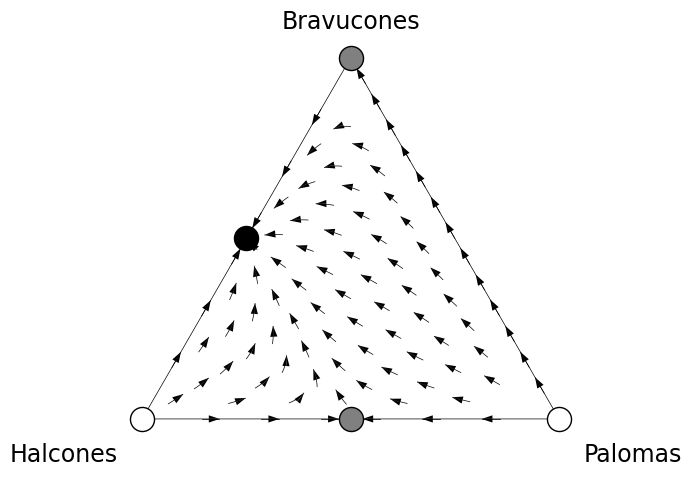
\includegraphics[width=0.7\textwidth]{ej2_hpb.png}
    \caption{Simplex para el juego de halcones, palomas y bravucones.} 
    \label{fig:ej2_hpb}
\end{figure}

\subsection*{Halcones, palomas y vengativos}

Ahora, tenemos un juego con la siguiente matriz de pagos

\begin{equation*}
    A =
\begin{pmatrix}
\frac{G-C}{2} & G & \frac{G-C}{2} \\[6pt]
0 & \frac{G}{2} & \frac{G}{2} \\[6pt]
\frac{G-C}{2} & \frac{G}{2} & \frac{G}{2} \\
\end{pmatrix}
\end{equation*}

Resolvemos de la misma forma que antes y llegamos al siguiente conjunto de ecuaciones
\begin{align}
    f_h &= \frac{G-C}{2}+\frac{G+C}{2}p \\
    f_p &= \frac{G}{2}(1-h), \\
    f_v &= \frac{G}{2}-\frac{C}{2}h, \\
    \bar{f} &= \frac{C}{2}h^2-Ch+Chp+\frac{G}{2}.
\end{align}
Luego, las ecuaciones de replicador son  
\begin{align}
    \dot{h} &= h\left(-\frac{C}{2}h^2-Chp+Ch+\frac{G+C}{2}p-\frac{C}{2} \right), \\
    \dot{p} &= hp\left(-\frac{G}{2}+C-\frac{C}{2}h-Cp \right).
\end{align}

Los puntos fijos del sistema se obtienen igualando a cero las ecuaciones del replicador. En este caso tenemos 3 puntos fijos para el sistema $(1,0,0)$, $(\frac{G}{C},1 - \frac{G}{C},0)$ y el punto $(0,p,1-p)$. Este último, punto fijo, es un punto fijo para cualquier valor de $p$ dado que $h$ se encuentra multiplicando a ambas ecuaciones del replicador.

Para analizar la estabilidad de los puntos fijos, calculamos la matriz jacobiana del sistema 
\begin{equation}
    J =
\begin{pmatrix}
-\frac{3}{2}Ch^2 - 2Chp + 2Ch + \frac{G+C}{2}p - \frac{C}{2} & -Ch^2 + \frac{G+C}{2}h \\[6pt]
-\frac{G}{2}p + Cp - Chp - C p^2  &  -\frac{G}{2}h + Ch - \frac{C}{2} h^2 - 2Chp \\
\end{pmatrix},
\end{equation}
y la evaluamos en los puntos fijos encontrados, nuevamente suponemos que $C > G$.

\begin{equation}
J |_{\left(1,0,0\right)} =
\begin{pmatrix}
    0  & \frac{G-C}{2} \\
    0  & \frac{C-G}{2}
\end{pmatrix} \hspace{1cm} \text{Punto fijo inestable.}
\end{equation}

\begin{equation}
J |_{\left(\frac{G}{C},1-\frac{G}{C},0\right)}=
\begin{pmatrix}
    0  & -\frac{1}{2}\frac{G^2}{C} + \frac{G}{2} \\
    \frac{1}{2}\frac{G^2}{C} - \frac{G}{2}       & \frac{G^2}{C} - G
\end{pmatrix} \hspace{1cm} \text{Punto fijo estable.}
\end{equation}

Ahora evaluamos sobre la recta de $h=0$

\begin{equation}
J |_{\left(0,p,1-p\right)} =
\begin{pmatrix}
    \frac{G+C}{2}p - \frac{C}{2}  & 0 \\
    p\left(-\frac{G}{2} + C - Cp\right)       & 0
\end{pmatrix} \hspace{1cm} \text{Acumulación de equilibrios.}
\end{equation}

En este último caso, la acumulación de equilibrios es estable si $p<\frac{C}{G+C}$ e inestable en caso contrario.


Finalmente, graficamos el simplex para $G = 1$ y $C = 2$ donde se grafica en blanco el puntos inestable, en negro el punto estable y la linea punteada la acumulación de equilibrios estables. Luego, vemos que el sistema tiende, en base a las poblaciones iniciales, al equilibrio estable en el punto $(\frac{G}{C},0,1-\frac{G}{C}) = (0.5,0.5,0)$ o al equilibrio sobre la recta $(0,p,1-p)$.

\begin{figure}[h]
    \centering
    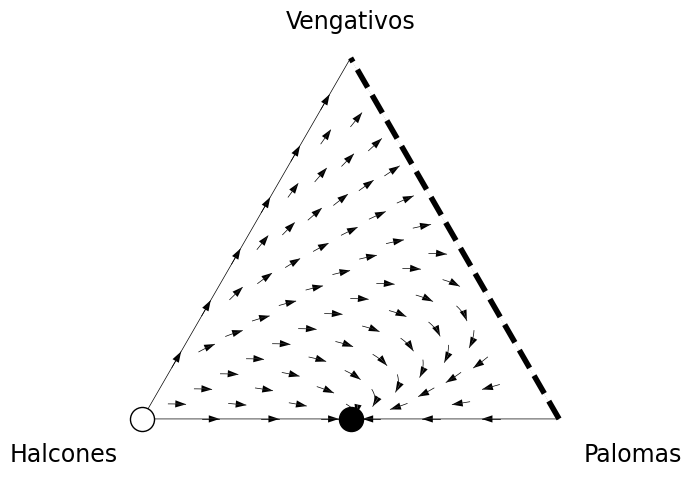
\includegraphics[width=0.7\textwidth]{ej2_hpv.png}
    \caption{Simplex para el juego de halcones, palomas y vengativos.} 
    \label{fig:ej2_hpv}
\end{figure}

\section*{Ejercicio 3 - Dilema del prisionero multijugador}

En primer lugar, comprendamos bien la tabla de payoff del enunciado. En dicha tabla, cada columna representa la cantidad de jugadores que cooperan. Es decir la primer columna da los payoff para un jugador que decide cooperar o no cooperar dado que hay 0 coperadores y n-1 defectores. La segunda columna da los payoff para un jugador que decide cooperar o no cooperar dado que hay 1 coperador y n-2 defectores y así sucesivamente. 

Sabemos que el dilema del prisionero para dos jugadores tiene dos reglas fundamentales
\begin{itemize}
    \item Individualmente, la estrategia dominante es defraudar. Por lo tanto, defraudar debe ser la mejor opción independientemente de lo que haga el otro jugador.
    \item La cooperación colectiva es mejor que la defraudación colectiva. Es decir, si ambos jugadores cooperan, ambos obtienen un payoff mayor que si ambos defraudan.
\end{itemize}

Ahora, queremos extrapolar estas reglas para el dilema del prisionero multijugador. Por lo tanto, como dijimos, la estrategia dominante es defraudar, luego defraudar debe ser la mejor opción independientemente de lo que hagan los otros jugadores, lo cual se traduce en 
\begin{equation}
    D_i > C_i \hspace{1cm} \forall i.
\end{equation}

Por otro lado, la cooperación colectiva es mejor que la defraudación colectiva, con lo cual podemos ver que $C_{n-1}$, es decir la paga cuando todos cooperan tiene que ser mayor que la paga cuando todos defraudan $D_0$, osea $C_{n-1} > D_0$.

Por último, veamos que para establecer una relación entre los coeficientes que quedan, podemos pensar que mientras más jugadores coperen mejor será la paga para todos, lo cual implica que $C_i > D_{i-1}$, hasta el punto en que si todos cooperan se obtiene la mejor paga, lo cual solo es superado por $D_{n-1}$ donde todos cooperan salvo uno que defrauda a todos.

Otra forma de pensarlo es que si un jugador coopera y los demás defraudan, el jugador que coopera debería tener una paga menor cuantos más jugadores defrauden. En el caso extremo en que todos defraudan, salvo uno que coopera, este último debería tener la peor paga (es un chivo expiatorio). 

Por lo tanto, las relaciones que deben cumplir los coeficientes son
\begin{equation}
    D_{n-1} > C_{n-1} > D_{n-2} > \dots > D_1 > C_1 > D_0 > C_0,
\end{equation}
donde vemos que se recupera el dilema del prisionero para dos jugadores ya que en el juego original $D_1 = 0$ años de cárcel, $C_1 = 1$ año, $D_0 = 6$ años, $C_0 = 10$ años de cárcel. Es decir, se satisface $D_1 > C_1 > D_0 > C_0$ (recordemos que la mejor paga en este caso es la menor cantidad de años de cárcel con lo cual es consistente).


%\bibliographystyle{plain} % Estilo de bibliografía
%\bibliography{bibliography}    % Nombre de tu archivo .bib sin la extensión

\end{document}